\documentclass{standalone}

\usepackage[siunitx,americanvoltages, europeanresistors,americancurrents]{circuitikz}
\usepackage{color}
\usepackage{graphicx}%Für Grafiken
\usepackage{rotating} % lässt Grafiken rotieren
\usepackage{mathtools}% mathematische Werkzeuge
\usepackage{amsmath}% Mathetools
\usepackage{amsfonts}% Mathetools
\usepackage{physics}
\usepackage{amssymb}% Symbole wie Natürliche Zahlen
\usepackage{geometry}
\usepackage{caption} % Unter-/Überschriften für Bilder, Grafiken und Tabellen
\usepackage{tikz}
\usepackage{amsthm}

% tikz libraries
\usetikzlibrary{arrows}
\usetikzlibrary{3d}
\usetikzlibrary{angles, quotes, shapes, decorations.markings, calc, arrows.meta}

% mathmatical commands
\newcommand{\AAA}{\mathbf{A}}
\newcommand{\R}{\mathbb{R}}
\newcommand{\N}{\mathbb{N}}
\newcommand{\p}{\mathcal{P}}
\newcommand{\I}{\infty}
\newcommand{\ve}{\varepsilon}
\newcommand{\vp}{\varphi}

\begin{document}
	Function:
 	\begin{equation}
		\left(D(\alpha) \cdot \alpha\right) \cdot \mathbf{e_1}
   	\end{equation}
	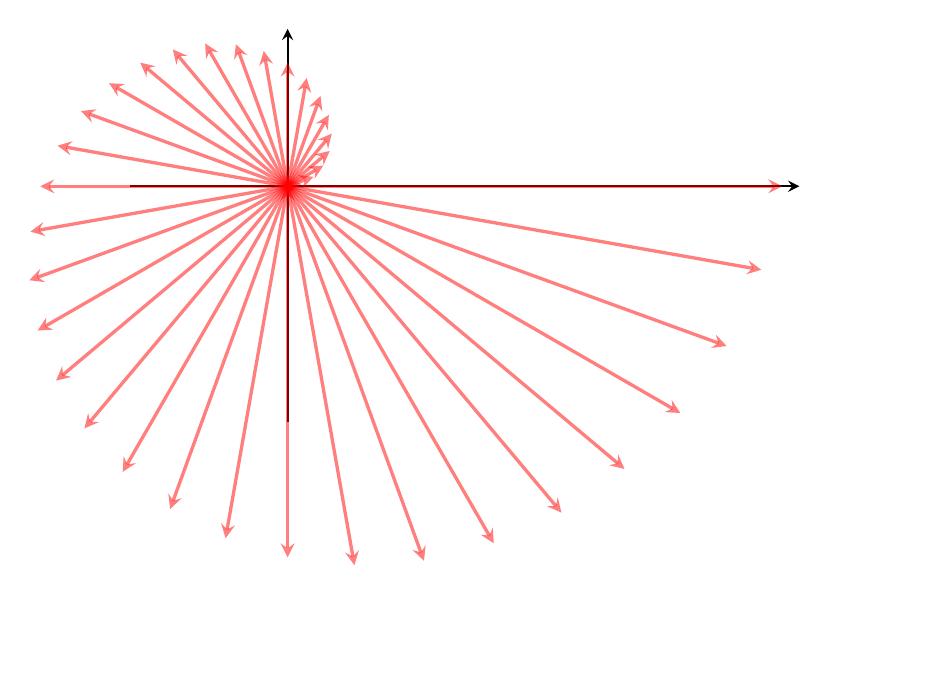
\begin{tikzpicture}[>=stealth]
		% regulation: (alpha * D(alpha)) * e_1
		\draw[color=white] (-2,-6) rectangle (8,2);
		\draw[->,thick] (-2,0) -- (6.5,0);
		\draw[->,thick] (0,-3) -- (0,2);
		\foreach \i in {0,10,...,360}{
			\draw[->,color=red,opacity=.5,very thick] (0,0) -- ({\i*pi/180*cos(\i)},{\i*pi/180*sin(\i)});
		}
	\end{tikzpicture}
	
\end{document}
